\documentclass[conference]{IEEEtran}
\IEEEoverridecommandlockouts
% The preceding line is only needed to identify funding in the first footnote. If that is unneeded, please comment it out.
\usepackage{cite}
\usepackage{amsmath,amssymb,amsfonts}
\usepackage{algorithmic}
\usepackage{graphicx}
\usepackage{textcomp}
\usepackage{xcolor}
\def\BibTeX{{\rm B\kern-.05em{\sc i\kern-.025em b}\kern-.08em
    T\kern-.1667em\lower.7ex\hbox{E}\kern-.125emX}}

\begin{document}

\title{RAISE: A Research-Driven, AI-First Software Engineering Framework for High-Compliance Environments}

\author{\IEEEauthorblockN{Gabriel Amazonas}
\IEEEauthorblockA{\textit{Founder \& Engineer} \\
\textit{Impacte}\\
Rio de Janeiro, Brazil \\
gabriel@impacte.tech}
}

\maketitle

\begin{abstract}
As Large Language Models (LLMs) increasingly automate code generation, the primary constraint in software engineering is shifting from implementation velocity to contextual accuracy and regulatory compliance. Traditional Agile methodologies, designed for human-centric coding, often fail to leverage the full capacity of AI agents or manage their stochastic risks. This paper proposes RAISE (Research-Driven AI-First Software Engineering), a novel workflow framework designed for hyper-growth, high-compliance financial environments. RAISE decouples execution from governance, assigning code synthesis to specialized AI agents while shifting human effort toward ``high-value research''---defining problems, validating architecture, and managing economic efficiency. We present a reference implementation using a heterogeneous multi-model stack (orchestrating Reasoning, Coding, and Infrastructure models) and a ``Policy-as-Code'' governance gate that ensures deterministic quality in an AI-first ecosystem.
\end{abstract}

\begin{IEEEkeywords}
Software Engineering, Artificial Intelligence, Large Language Models, Compliance, DevOps, FinTech
\end{IEEEkeywords}

\section{Introduction}
The software engineering discipline is currently undergoing a paradigm shift comparable to the transition from Waterfall to Agile. For the past two decades, methodologies like Scrum and Extreme Programming (XP) have optimized for \textit{human velocity}---reducing the time it takes for a human to write, test, and deploy code. However, the emergence of Large Language Models (LLMs) effectively drives the cost of producing functional code toward zero.

In this new era, the bottleneck is no longer ``how fast can we write code,'' but ``how accurately can we define the problem.'' Failing to integrate AI agents into the core engineering loop represents a massive opportunity cost for modern enterprises. Yet, unbridled AI adoption poses significant risks, particularly in high-compliance sectors (e.g., Fintech, Healthcare), where ``hallucinations'' or security vulnerabilities are unacceptable.

We introduce \textbf{RAISE}, a framework that restructures the software development lifecycle (SDLC) around two core principles:
\begin{enumerate}
    \item \textbf{AI-First Execution:} LLMs are treated not as assistants, but as primary agents of implementation.
    \item \textbf{Research-Driven Oversight:} Human engineering time is reallocated from syntax generation to \textit{research}---investigating emerging tools, defining architectural boundaries, and optimizing cost models.
\end{enumerate}

This paper outlines the theoretical structure of RAISE, its ``Tripartite'' workflow model, and a reference implementation that has been deployed to optimize engineering velocity in high-regulatory contexts.

\section{Theoretical Foundation}

The RAISE framework is built upon the premise that LLMs and Small Language Models (SLMs) will continuously improve at routine engineering tasks. Consequently, human intervention must move ``up the stack'' to areas where AI lacks training data or context.

\subsection{The Research-Driven Human Contribution}
Current LLMs suffer from ``knowledge cutoffs''---they are unaware of the latest frameworks, security vulnerabilities, or internal company constraints released after their training date. In the RAISE model, the human engineer's role is defined as:
\begin{itemize}
    \item \textbf{Methodology Innovation:} Discovering new architectural patterns that AI models have not yet ingested.
    \item \textbf{Contextual Injection:} Providing the AI with ``fresh'' research regarding industry standards (e.g., new ISO regulations) or project-specific constraints.
    \item \textbf{Economic Optimization:} Managing the ``token economics'' of the development lifecycle.
\end{itemize}

\subsection{The AI-First ``Agentic'' Shift}
Unlike ``AI-Assisted'' workflows (where a human writes code and AI suggests completions), RAISE is ``AI-First.'' The AI generates the initial implementation, documentation, and tests based on human-defined specifications. The human acts as a \textit{Reviewer} and \textit{Architect} rather than a \textit{Writer}.

\section{The RAISE Framework Architecture}

The framework operates on a \textbf{Heterogeneous Model Orchestration} architecture, leveraging a ``Tripartite'' workflow that assigns distinct cognitive roles to specific model classes based on their capabilities (e.g., reasoning depth vs. context window size).

\subsection{The Tripartite Workflow}
The SDLC is divided into three distinct phases, each mediated by a specialized AI agent (See Fig.~\ref{fig1}).

\subsubsection{Strategic Layer (Ideation \& Logic)}
\begin{itemize}
    \item \textbf{Objective:} Define ``what'' to build without hallucinating ``how.''
    \item \textbf{Agent Role:} \textit{The Strategist.} (Implementation: \textbf{Large Reasoning Model}).
    \item \textbf{Process:} The human engineer inputs raw business hypotheses. The agent refines these into \textbf{Document-as-Code (DaC)} artifacts---specifically Product Requirement Documents (PRD) and Requests for Comments (RFC). This ensures that ambiguity is resolved \textit{before} implementation begins.
\end{itemize}

\subsubsection{Execution Layer (Implementation)}
\begin{itemize}
    \item \textbf{Objective:} Convert DaC artifacts into functional, compliant code.
    \item \textbf{Agent Role:} \textit{The Builder.} (Implementation: \textbf{High-Context Coding Model}).
    \item \textbf{Configuration:} The agent operates under strict ``Rules of Engagement'' defined in a semantic governance repository. These rules mandate adherence to internal style guides and prohibit ``magic numbers'' or undocumented logic.
\end{itemize}

\subsubsection{Governance \& Infrastructure Layer}
\begin{itemize}
    \item \textbf{Objective:} Deployment, documentation, and cost management.
    \item \textbf{Agent Role:} \textit{The Librarian.} (Implementation: \textbf{Long-Context Infrastructure Agent}).
    \item \textbf{Process:} This agent manages Infrastructure-as-Code (IaC), updates internal wikis, and analyzes token usage logs to recommend cost-saving optimizations.
\end{itemize}

% FIGURE PLACEHOLDER
% You must upload a file named 'raise_diagram.png' (or jpg) to your project folder.
\begin{figure}[htbp]
\centerline{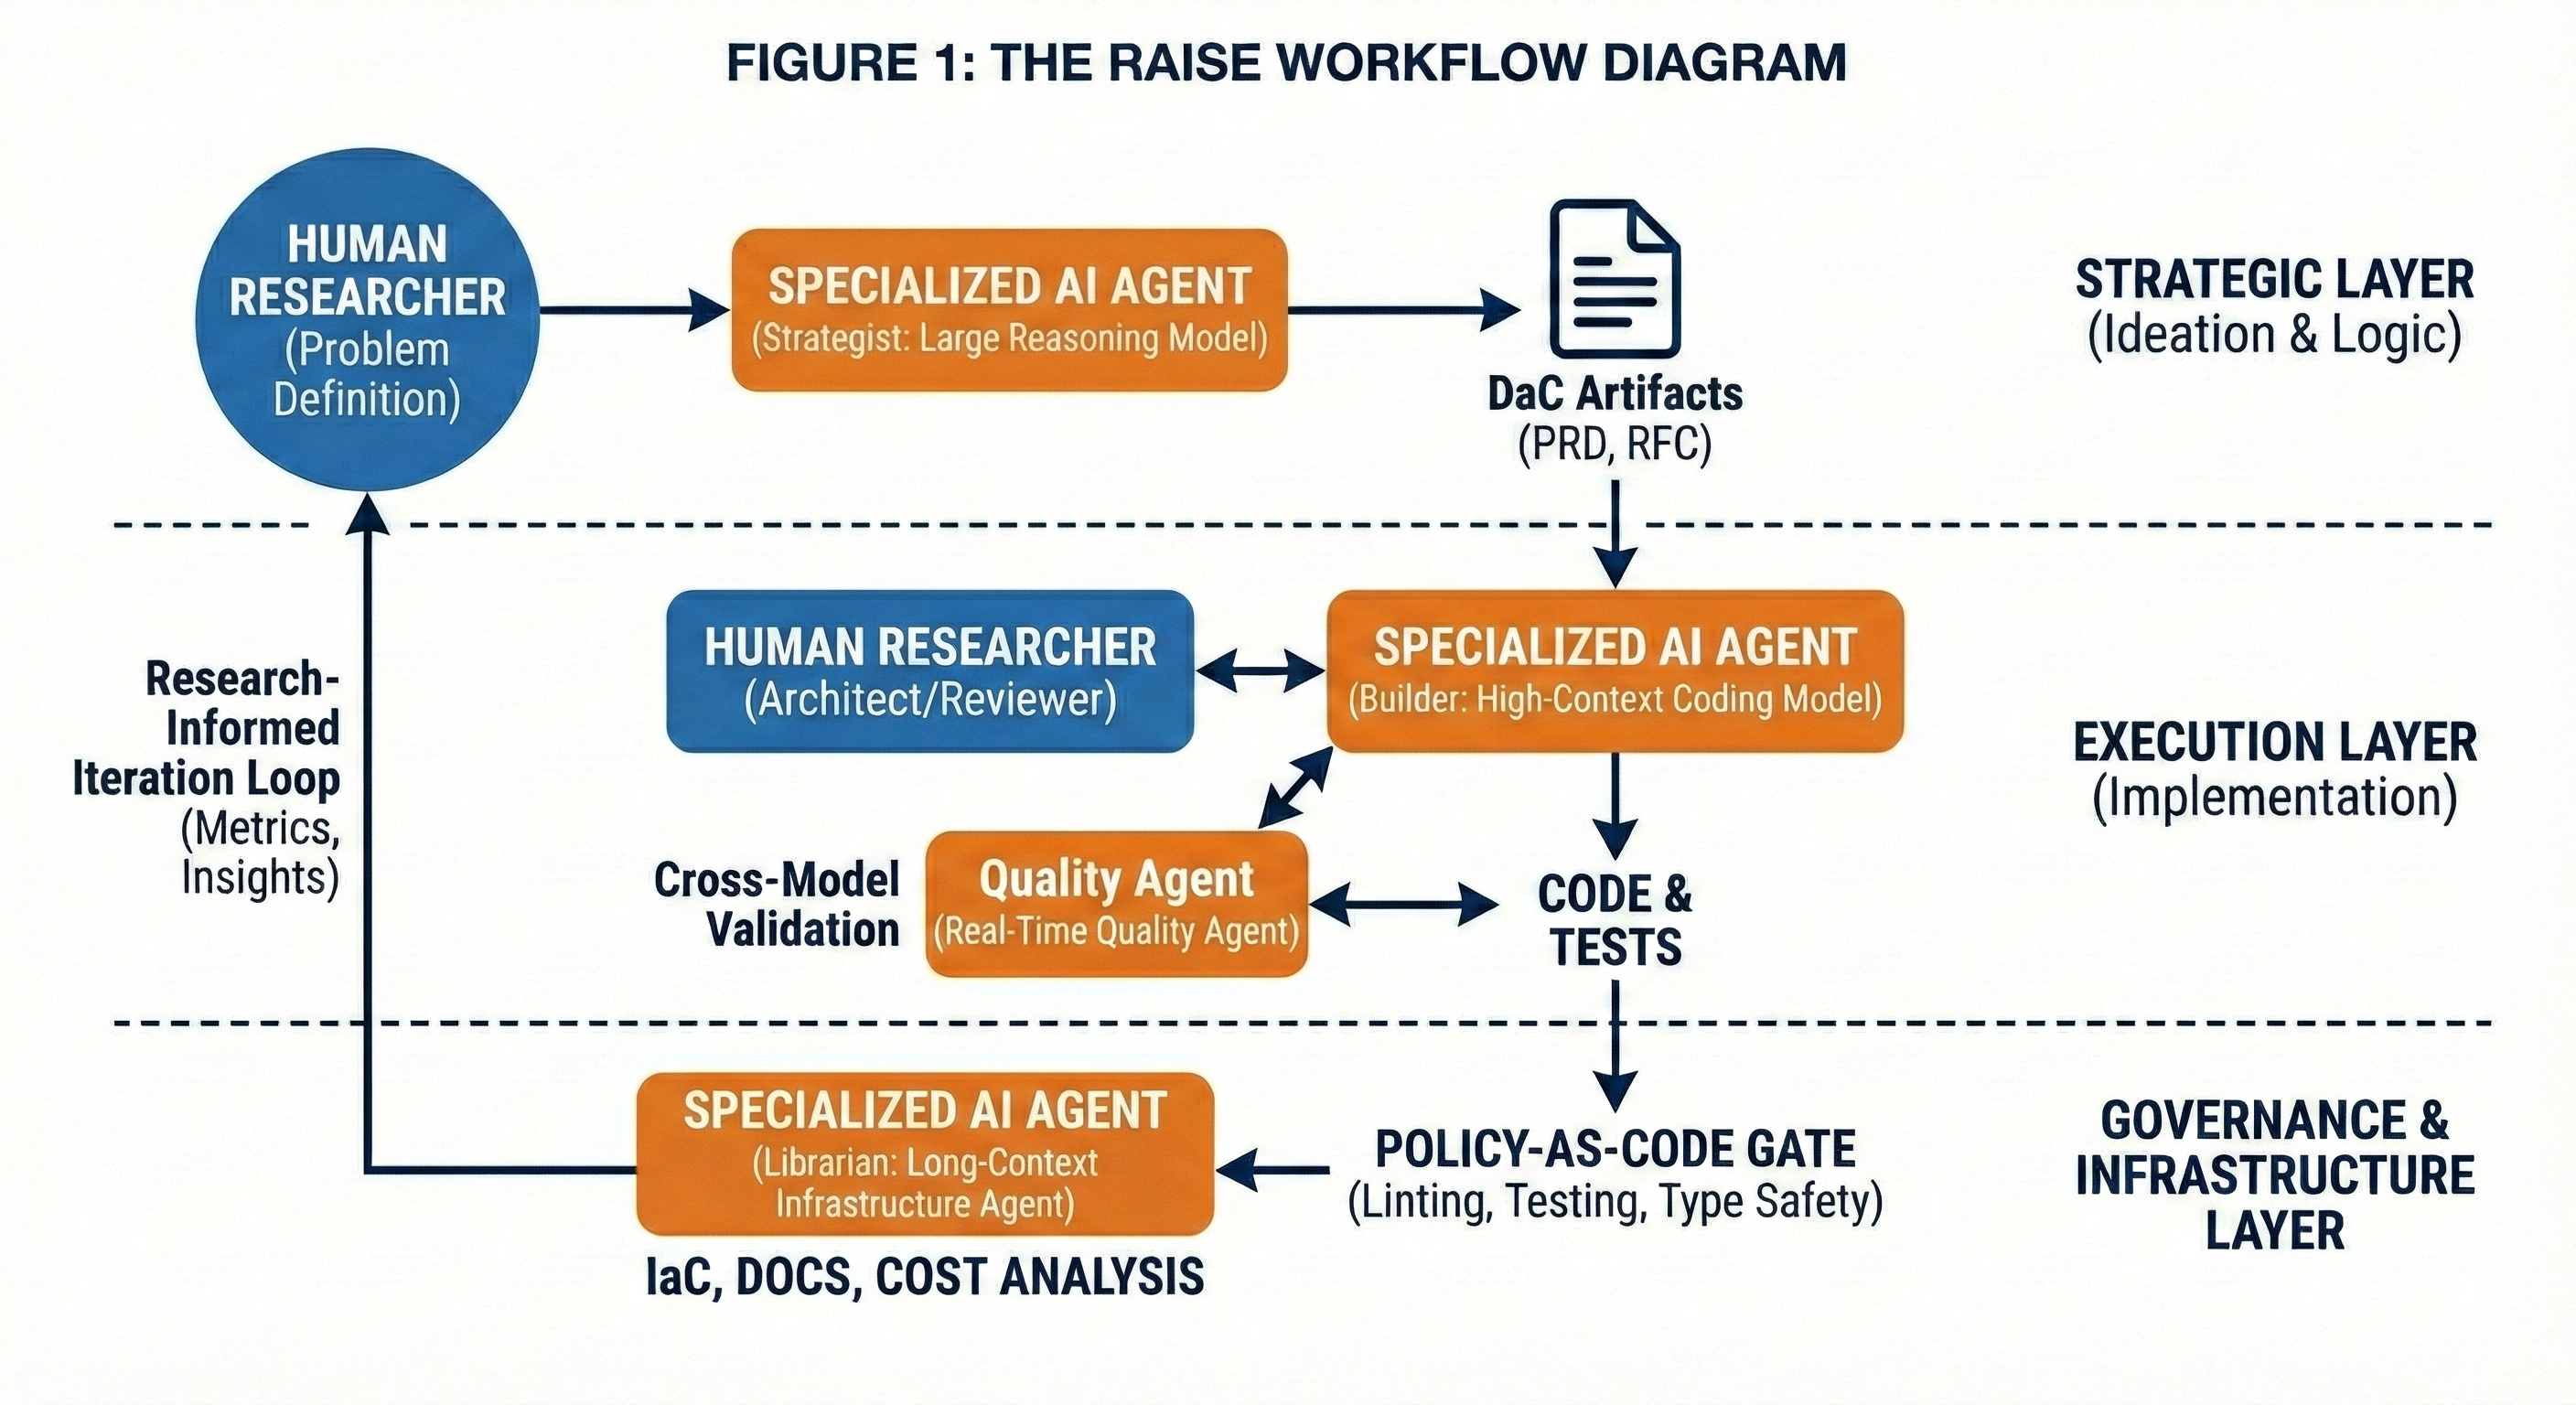
\includegraphics[width=\columnwidth]{raise_diagram.png}}
\caption{The RAISE Workflow Diagram. The process illustrates the flow of information between Human Researchers (Blue nodes) and Specialized AI Agents (Orange nodes), highlighting the cyclical nature of the ``Research-Informed Iteration'' loop.}
\label{fig1}
\end{figure}

\subsection{The Governance Gate (Policy-as-Code)}
To safely deploy AI-generated code in a regulated environment, RAISE imposes a ``Zero-Trust'' verification pipeline.

\begin{itemize}
    \item \textbf{Cross-Model Validation:} Code written by the \textit{Builder Agent} is reviewed by a separate \textit{Quality Agent}. This adversarial review process catches logic errors that a single model might miss.
    \item \textbf{Automated Quality Gates:} A pre-commit pipeline enforces deterministic checks:
    \begin{enumerate}
        \item \textit{Linting:} Automated formatting enforcement.
        \item \textit{Testing:} Mandatory code coverage thresholds for all branches and functions.
        \item \textit{Type Safety:} Strict static compilation checks.
    \end{enumerate}
\end{itemize}

\section{Implementation and Configuration}

We present a reference implementation of RAISE designed for a modern web stack, though the principles remain agnostic to the underlying technology.

\subsection{Deterministic Agent Configuration}
To prevent the ``drift'' often associated with LLM code generation, the framework utilizes context-aware instruction sets.
\begin{itemize}
    \item \textbf{Context-Aware Governance Rules:} Defines the ``Constitution'' for the AI agent. It explicitly forbids the agent from modifying code without first analyzing the existing architectural patterns.
    \item \textbf{Chain-of-Thought Audit Logs:} A logging pattern where the agent must document its reasoning in a dedicated artifact. This provides a traceable audit trail for compliance officers, explaining \textit{why} a specific algorithmic decision was made.
\end{itemize}

\subsection{The Testing Architecture}
RAISE mandates a Test-Driven Development (TDD) cycle where the AI generates tests \textit{before} or \textit{alongside} functionality.
\begin{itemize}
    \item \textbf{Unit \& Integration:} The pipeline is configured to block any commit that lowers the global coverage threshold below acceptable standards (e.g., 80\%).
    \item \textbf{End-to-End (E2E):} Tests are generated to validate critical user flows, ensuring that AI-generated UI changes do not break business logic.
\end{itemize}

\subsection{Economic Monitoring}
The framework introduces \textbf{Token Cost Analysis} as a standard engineering metric.
\begin{itemize}
    \item \textbf{Pre-Task Estimation:} Engineers are trained to estimate token load before complex queries.
    \item \textbf{Model Routing:} Routine tasks (documentation formatting) are routed to lower-cost models, while complex architectural reasoning is routed to specialized ``Reasoning Models,'' optimizing the return on compute spend.
\end{itemize}

\section{Discussion and Impact}

\subsection{Preliminary Pilot Results}
In early-stage deployments of the RAISE framework within a global-scale financial environment, we observed a significant acceleration in software delivery metrics. By moving the "Code Review" phase to an asynchronous, AI-first model, the deployment cycle time for complex features was reduced from months to weeks---representing a velocity increase of over 500\%. This acceleration suggests that the primary friction in traditional regulated software engineering is not implementation difficulty, but the latency introduced by synchronous human coordination \cite{b6}.

\subsection{The Shift in Developer Roles}
Implementing RAISE transitions the engineering workforce from ``Code Producers'' to ``System Architects.'' As noted by recent studies on generative AI, the developer's role is shifting from syntactic generation to high-level system design and intent specification \cite{b4}.
\begin{itemize}
    \item \textit{The Junior Engineer:} Focuses on reviewing AI output and learning through ``reverse engineering'' the AI's solutions.
    \item \textit{The Senior Engineer:} Focuses on ``Prompt Engineering Strategy'' and defining the regulatory boundaries within which the AI must operate.
\end{itemize}

\subsection{Compliance in Fintech}
In financial sectors, the ``Black Box'' nature of AI is a liability \cite{b5}. RAISE mitigates this through the \textbf{Document-as-Code} pillar. By forcing the AI to generate human-readable PRDs and ADRs (Architecture Decision Records) \textit{before} coding, the framework creates a paper trail that satisfies audit requirements, effectively treating the AI as a junior employee whose work is fully logged and reviewed.

\section{Conclusion}

The RAISE framework offers a pragmatic path for integrating high-performance AI agents into regulated software environments. By acknowledging the strengths of specific models---Strategic Reasoning, Code Synthesis, and Infrastructure Management---and binding them within a strict ``Policy-as-Code'' governance structure, organizations can achieve the velocity promised by AI without sacrificing the stability demanded by the financial industry.

Future work will focus on automating the ``Context Injection'' layer, allowing agents to autonomously ``research'' internal documentation without human prompting.

\begin{thebibliography}{00}

\bibitem{b1} G. Amazonas, ``RAISE: Research-Driven AI-First Software Engineering Repository,'' GitHub, 2025. [Online]. Available: https://github.com/GabrielAmazonas/raise.

\bibitem{b2} A. Vaswani et al., ``Attention Is All You Need,'' in \textit{Advances in Neural Information Processing Systems}, vol. 30, 2017. [Online]. Available: https://arxiv.org/abs/1706.03762.

\bibitem{b3} S. Maatouk et al., ``Large Language Models (LLMs): Deployment, Tokenomics and Sustainability,'' Huawei, University of Ottawa, 2024. [Online]. Available: https://arxiv.org/abs/2405.17147.

\bibitem{b4} OpenAI et al., ``Early science acceleration experiments with GPT-5,'' OpenAI, Harvard University, University of Cambridge, 2025. [Online]. Available: https://arxiv.org/abs/2511.16072.

\bibitem{b5} Z. Ziegler et al., ``Research: Quantifying GitHub Copilot's impact on developer productivity and happiness,'' \textit{GitHub Research}, 2024. [Online]. Available: https://github.blog/2023-06-27-research-quantifying-github-copilots-impact-on-developer-productivity-and-happiness/.

\bibitem{b6} P. Ralph et al., ``Generative AI and Empirical Software Engineering: A Paradigm Shift,'' \textit{arXiv preprint arXiv:2502.08108}, 2025.

\bibitem{b7} A. A. C. et al., ``10 Benefits and 10 Challenges of Applying Large Language Models to Software Acquisition,'' \textit{Software Engineering Institute (SEI) Blog}, Carnegie Mellon University, 2024.

\bibitem{b8} Y. H. et al., ``An Empirical Study on Challenges for LLM Application Developers,'' \textit{arXiv preprint arXiv:2408.05002}, 2024.

\end{thebibliography}

\end{document}